\chapter{System Analysis}
\label{chap:sysAnalysis}

% Goal of chapter:
This chapter formulates characteristics of the two considered systems and their combination, to answer subquestion 2:

\begin{itemize}
\item What characteristics does a vessel system have that integrates automated assembly with configuration dependent control?
\end{itemize}

Answering this question will bring better understanding of the meaning of "a system that performs self-assembly" and "a multi-robot-assembly performing collaborative and coordinated control". The aim is to look beyond the design solutions from the projects described in the previous secion, and create a broader view on the design spectrum. 

% Structure of chapter
The first section explores characteristics of systems performing automated assembly (section \ref{analysisReconfiguration}) and configuration dependent control (section \ref{analysisConfigAdaptation}).
This chapter concludes by mapping system characteristics as a result of integrating both behaviors (section \ref{analysisCombined}). 

This section uses various external sources to aid formulation of characteristics, some of which have been discussed in the previous chapter. 
The overall approach is to distinct generalized system characteristics as well as a narrowed down set of solutions that can be considered more feasible to perform in commercial applications, also taking into account design choices of other projects. 


\section{Analysis of first required behavior: Automatic vessel platform reconfiguration}
\label{analysisReconfiguration}

Automated modular vessel platform reconfiguration systems can be categorized as a more general "modular reconfigurable robot" system. 
Modular reconfigurable vessel systems can be evaluated from a non-maritime perspective, so where we are not directly focussing on vessels, but on more general modular reconfigurable robot (MRR) systems. \citet{seo2019modular} describes an MRR system as made up of many repeated modules (or units) that can be rearranged- or can rearrange themselves into different configurations depending on the task the robot is to solve at the time. The key characteristic of such systems is described as adaptability of hardware structure to suit a given task or environment. MRR systems differentiate themselves from normal robot systems by determining and executing a course of action, to change it's configuration. 

Various requirements of floating MRR systems were identified during the course of the project. Some approaches originating from sources about robotics in general were broader than approaches encountered in sources about modular vessel platforming. This section aims to conclude with two things. Firstly, it searches for fundamental characteristics of an automatic reconfiguring vessel platforming system. Secondly, the whole range of design choices and approaches is scoped down to a set that is expected to have the highest commercial feasibility. This is based on design choices of prior projects, supplemented with the authors argumented vision. 
During elaboration on system characteristics, prior projects will be discussed, more specifically, how they solved their challenges and in which characteristics did this result in. Automated vessel platform reconfiguration characteristics are discussed in 2 aspects; Strategies and Actuation. 



\subsection{Strategies}
\citet{yim2007modular} describes a taxonomy of architectures of modular robots, which is adopted to the use case of surface vessel platform reconfiguration. MRR system architectures are classified in three generally observed classes. They are described as follows \cite{yim2007modular}
\begin{itemize}
	\item \textbf{Lattice Reconfiguration Architectures} have units that are arranged and connected in some regular, three-dimensional pattern, resulting in a relatively simple and easily scalabe system. 
	\item \textbf{Chain or Tree Architectures} have	units that are connected together in a string or tree topology. This chain or tree can fold up to become space filling, but the underlying architecture is serial.
	\item \textbf{Mobile Architectures} have units that use the environment to maneuver around and can either hook up to form complex chains or lattices or form a number of smaller robots that execute coordinated movements and together form a larger	“virtual” network. 
\end{itemize}

We can see that \citet{o2014self} uses a lattice reconfiguration architecture in the horizontal surface plane (figure \ref{fig:wuh_assembly_planning}). Roboat shows L configurations in various publications, which can be considered a chain architecture, as configurations are used that do not fit in a repeating (lattice) pattern. Roboat reduces the amount of possible configurations by utilizing the square shape of the vessels to reduce the amount of orientations to steps in relative angle of 90 degrees.

Another classification can be found in the way structures are (re)configured. \citet{yim2007modular} distincts two approaches:
\begin{itemize}
	\item \textbf{Deterministic Reconfiguration} uses modules that are purposely manipulated to a target location.
	\item \textbf{Stochastic Reconfiguration} relies on statistics of a set of modules to configure in a more desirable configuration. System design is aimed to reach acceptable configuration without the need of predefined reconfiguration planning.
\end{itemize}

Stochastic reconfiguration can be achieved with very limited functionality per module. Due to robot simplicity, this approach can very desirable on micro scale which can be scaled to great numbers.
Deterministic reconfiguration needs more functionality embedded in a module. This system requires an agent that makes some form of plan, which is then to be executed. As a plan is formed and executed, this approach does give the opportunity to give more guarantees that a desired configuration is reached within a timespan. 

Due to technological advances, communication and computational hardware has become increasingly affordable. If the amount of modules in a system is relatively small, then equipping each individual with communication, computation and control systems is feasible. This allows creation of networks of robots that can share information, collaborate, negotiate and utilize benefits of all sorts of layered control architectures. Both \citet{o2014self} and Roboat utilize a deterministic approach to reach assembly. 

A common approach to solving the task of deterministic reconfiguration is dividing it in several tasks. \citet{o2014self} describes the following states to reach assembly:

\begin{itemize}
	\item Generation of desired configuration. \citet{o2014self} describes the result as a blueprint with a map of relative boat positions. 
	\item Connecting sequence selection. An entity selects a sequence in which the assembly is to happen. 
	\item Positioning of a module.  A trajectory of a vessel to an assembly location is generated and realized by actuators. 
	\item Docking Sequence. As a vessel reaches a docking site within an area of acceptance, the docking sequence runs, which should finalize the docking of that vessel. 
\end{itemize}

\citet{o2014self} greatly illustrates how they formulated strategies for generating connection sequence and module positioning (figure \ref{fig:wuh_assembly_planning} and \ref{fig:wuh_assem_approach})
 \begin{figure}[h!]
	\centering
	\makebox[\textwidth][c]{
		\begin{minipage}{0.45\textwidth}
			\centering
			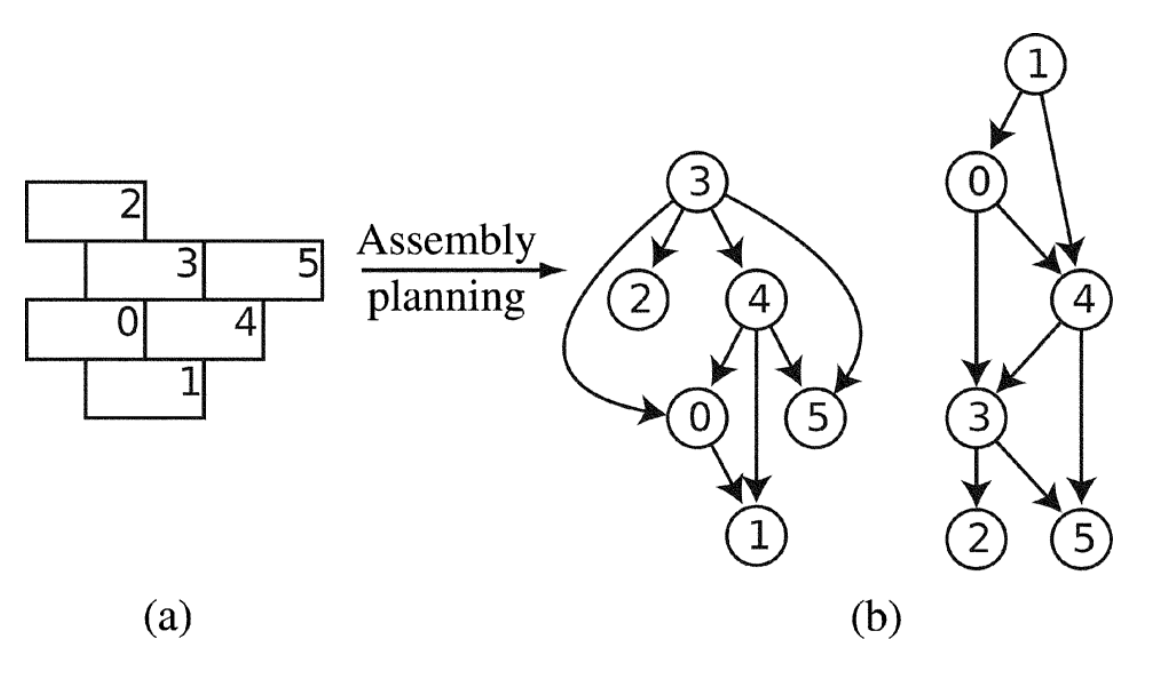
\includegraphics[width=0.95\textwidth]{img/wuh_assembly_planning}
			\caption{The assembly planning stage of \citet{o2014self}, showing desired platform blueprint (a) and two cannidate assembly sequences (b).}
			\label{fig:wuh_assembly_planning}
		\end{minipage}\hfill
		\begin{minipage}{0.45\textwidth}
			\centering
			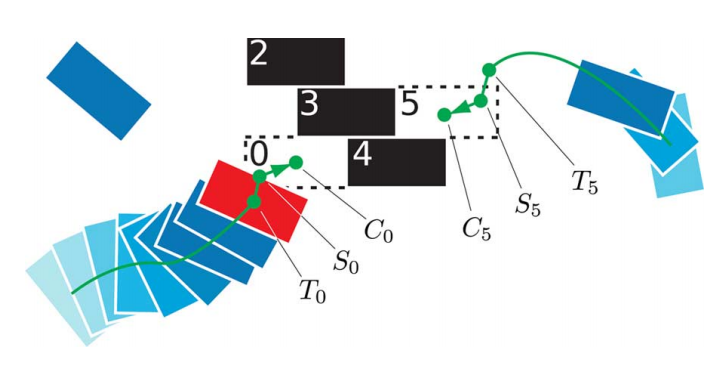
\includegraphics[width=0.95\textwidth]{img/wuh_assem_approach}
			\caption{The trajectory of assembling modules positioning to continue into a docking sequence \cite{o2014self}.}
			\label{fig:wuh_assem_approach}
		\end{minipage}
	}
\end{figure}

\subsection{Actuation}
Two tasks are identified that must be realized by actuators of the system:
\begin{itemize}
	\item means of relative repositioning modules during reconfiguration
	\item means of maintaining acceptable relative position between modules when connected
\end{itemize}

Altough these tasks can theoretically be done by a single system, \citet{seo2019modular} notices that MRR modules generally have two actuator systems to adress these tasks; a large main actuator to move itself with respect to other modules, and a smaller actuator that connects or disconnect two modules. 

The main actuator of MRR systems can be measured in nondimensional characteristic length, being "the number of modules that can be supported in a cantilever fashion under gravity"\cite{seo2019modular}. This measure is perhaps useful for some robotic systems, but does not make sense to use for vessel platforming systems, as gravitation is cancelled out by buoyancy and hydrodynamic forces. These forces are defined as \citet{fossen2011handbook}:
\begin{itemize}
	\item Buoyancy force due to the hydrostatic pressure (proportional to the displacement of the ship).
	\item Hydrodynamic force due to the hydrodynamic pressure (approximately proportional to the square of
	the relative speed to the water).
\end{itemize}

Vessel platforms are not considered excelling at tasks that require large speeds, but rather tasks that benefit from versatility, robustness  and low cost\cite{seo2019modular}. Vessels platforms with relatively low operational speeds can be classified as "Displacement Vessels" \citet{faltinsen2005hydrodynamics}
\begin{equation}
	Fn =  \frac{U}{\sqrt{gL}} < 0.4 \mbox{ }\mbox{ }\mbox{ }\mbox{ for vessels categorized as "Displacement Vessels"}
\end{equation} 

The nature of displacement vessels allow horizontal movement of masses (the ship itself and cargo) much higher with respect to robotic systems that lift, which results in a completely different order of magnitude of the ratio between propulsion and inertia. 
Vessel modules do need means of relocation with respect to other vessels with enough strength to overcome reasonable disturbances, such as wind or current. Further increasing the magnitude of forces that relocate the module reduces the achievable time that a module needs to relocate, which is also dependent on inertia and drag. Strength of main actuator and module mass are affected by various design choices, but optimal choices vary widely per use case. 
Systems that fulfull the task of moving the vessel in the surface plane come in many forms and configurations. Common actuators are propellers, rudders or fins. It is often considered desirable to have a set of actuators that allow imposing forces on all the three degrees of freedom independently, such that we can consider the module fully actuated. Figure \ref{fig:roboatAllocation} and \ref{fig:modularContainerAssembly} show actuator setups of the Roboat and \citet{o2014self}, which can both be considered fully actuated. 

 \begin{figure}[h!]
	\centering
	\makebox[\textwidth][c]{
		\begin{minipage}{0.45\textwidth}
			\centering
			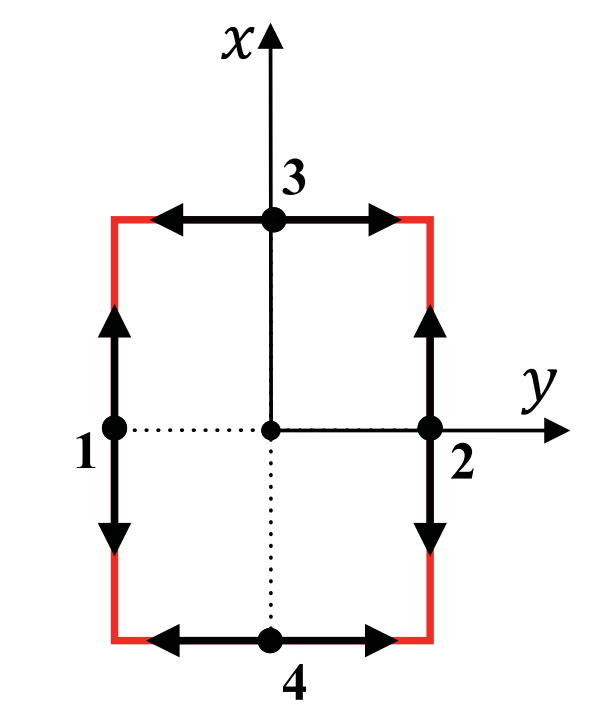
\includegraphics[width=0.75\textwidth]{img/roboatThrusterAllocationPlus}
			\caption{The "+" shaped thruster setup of Roboat \cite{wang2018design}}
			\label{fig:roboatAllocation}
		\end{minipage}\hfill
		\begin{minipage}{0.45\textwidth}
			\centering
			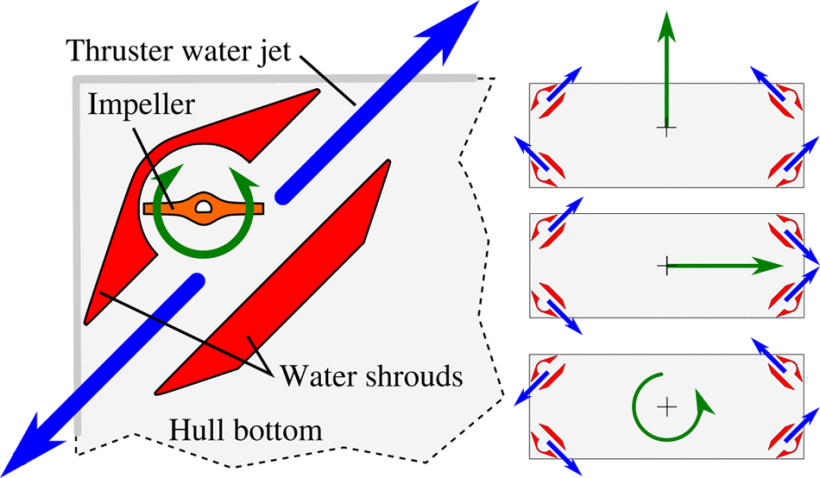
\includegraphics[width=0.9\textwidth]{img/TEMPMThrusterAllocation}
			\caption{The "x" shaped hruster setup of "Tactically expandable maritime platform module" \cite{o2014self}}
			\label{fig:modularContainerAssembly}
		\end{minipage}
	}
\end{figure}

A vessel platforming system needs means to maintain its configuration, which can be achieved using physical restraints that limit relative motion between modules for some period of operation. Movement of the platform as a whole can be desired, for instance when a vessel platform is performing a task of moving to a certain point or orientation. Undesired movement can be caused by disturbances. Alhough maintaining configuration of a vessel platform can theoretically be realized by the main actuators of the module, it is often seen that a second type of actuator is applied, specifically designed to reduce unwanted relative motion between modules by means of physical constraint. Generally once such systems are implemented, often by  mechanical \cite{mateos2019autonomous} \cite{o2014self} or magnetic \cite{kelly2019algorithms} means, the configuration is considered an assembly.


The application of MRR systems on vessel platforms is a niche which generally has specific goals, constraints, environments. The majority of the motion is on the surface plane, often allowing engineers to consider only three degrees of freedom. The environment already enforces some degree of dampening to the system, as various hydrodynamic dampening effects are always present on ships. Robots performing self-reconfiguration is a big topic, on which the most relevant concepts for vessel platforming are elaborated in this section. For further reading on general (not vessel platforming) MRR systems, consider \citet{yim2007modular} and \citet{seo2019modular} and references therein.



%"A key ability of MRR systems that differentiates them from normal robot systems is the
%This problem is referred to as
% and control." 


%More connecting methods can arise in the future, which do not fit a particular mentioned group. Hybrid systems are possible and can even %be more suitable to best exploit benefits of MRR systems for a particular application. 

%We consider a vessel system that self assembles a system with a connection mechanicm able to meet all prerequisites for this connecting mechanism to maintain acceptable relative motion. 
%Motion between connected vessels may be non neglectable, as was assumed in the case of \citet{paulos2015automated}. Their rope-like connections could change their stiffness by controlling tension in the cables that are part of their construction. The area of acceptance has been predicted and compared with success rate in their experimental setup. The connection protocol required the connecting vessels to be in constant relative position of one another. 


%\citet{mateos2019autonomous}'s ball joint connections between assembling vessels have a higher translational stiffness with respect to \cite{paulos2015automated}. The ball joints do however give almost no rotational stiffness between vessels. The ball joint latching system needs both vessels to approach one another at a small range of angles. the cone around the ball joint system helps to enlarge the area of acceptance, by physically guiding the relatively small joints to eachother. 


%Practically, both systems were able to perform vessel self assembly. Both systems will have benefits over one another, and there are even more solutions possible than the two described above. Choice of connection method and protocol is up to a designer, and optimal choices vary among applications. 

%What 



%\citet{seo2019modular} 


%\citet{seo2019modular} states: 
%"Here we will give examples of MRR systems in each architectural class. The intent is not to be exhaustive, but to find historically early %representative examples.
%"


%todo: map functions of the system. What is to be controlled and what not? There are more control tasks than generic ship control systems, which are to be discussed. 

%This section will discuss functions of general vessel systems. 
%Automation will be evaluated in four classes of functions as \citet{parasuraman2000model}. The classes of functions are as follows:
%\begin{enumerate}
%	\item information acquisition
%	\item information analysis
%	\item decision and action selection
%	\item action implementation
%\end{enumerate}
%Each of these functions can be automated independently. 

%In the context of 'ship control automation', the main function of a vessel system is considered the control of actuators to move the vessel. Operation of other functions are usually not the main focus. 
%A vessel controller able to realize a ship performing a succesful voyage might not be designed for loading and unloading a vessel, mainenance or fuel management.

%Vessel control systems can be equipped to manage tasks other than moving the vessel depending, but the core function usually contains motion control. 

%Generally communication, maintenance and other non manouvering jobs are not the scope when determining wether a vessel is automated or not. The nature of the controller of the ship's propulsion system determines automation. 

%Control may be achieved with a variety of systems that operate on different levels. 
%Consider a first system: Heading control of a vessel, achieved with a PID controller. Only one actuator (rudder) is controlled. The system controls actuation of the rudder, according to predefined laws for that operation. 
%Consider a second system: A vessel-system plans it's trajectory in a dynamic environment to arrive at a given destination, and controls actuators to realize this. 

%With respect to the former, system two will be more layered, equipped with more, sensors, actuators, and protocols, potentially performing more complex tasks. Yet, both systems have a controller that is responsible for a set of actuators. Both controllers decide and realize actuation for a given time. 
%-----

% DOUBLE ! \subsection{System A: automatic vessel platform assembly}
%With respect to the function of vessel motion control, another system function emerges in vessel platforming; assembly. 

%This means we are looking to automate vessels such that a present connecting system able to, partially or completely, prevent motion between vessels, thus forming a single body. Systems that connect vessels have requirements to perform reliably. The need of a specific relative motion between vessels varying over a connection-period is common, if not a must. 

%If the connection protocol was succesful, relative motion between vessels is restricted to some degree, or up to certain limits. Connections can be modeled as springs. Connectors with stiffness so high that relative motion between vessels 

% What does it mean to become a platform? What does this require?
%To consider vessels a platform, a method of connecting is required. This should be any tool that restricts or prevents relative motion between modules, up to certain limits. This can be of mechanical nature \citet{mateos2019autonomous}, or other means, such as with springs or magnets. % Roboat latching paper

%To call a system self-assembling: what is required?
%We need a vessel system that can manage orienting the vessel to come in range of acceptance of a connecting mechanism, as described above. Furthermore the ships need to satisfy demands that result from the specific latching system, such as time or contact force. 

%The self assembling features of a vessel system can generally be evaluated with indicators such as speed, reliability, energy consumption wear and ease of use, according to the demands of a use case. 

\section{Analysis of second required behavior: Configuration adaptive vessel platform control}
\label{analysisConfigAdaptation}

\subsection{Problem Description}
We have a team of $n$ modules connected into a platform. $n$ can vary through time as modules connect or disconnect. 
There exists an expression of the state of the platform expressed similar to single vessels as:

\begin{equation}
\eta_p = \begin{bmatrix} \textbf{p}^{n}_{p} \\[8pt]  \Theta_{np} \end{bmatrix} = \begin{bmatrix} x^{n}_{p} \\[8pt]  y^{n}_{p} \\[8pt] \Psi^n_p \end{bmatrix}
\end{equation}

\begin{equation}
\nu_p = \begin{bmatrix} \textbf{v}^{p}_{p/n} \\[8pt]  \omega^{p}_{p/n} \end{bmatrix} = \begin{bmatrix} u\\v\\r \end{bmatrix}
\end{equation}

Where $\eta_p$ and $\nu_p$ describe generalized positions and velocities of the platform coordinate system origin.  If the platform connections can be assumed rigid, a platform fixed coordinate system can be made that defines platform state in the above mentioned $\eta_p$ and $\nu_p$. Other definitions of platform state can be fixed to a single vessel, which does not assume rigid connections, or by coinciding the platform origin with its estimated overall centre of mass. Figure \ref{fig:bartned_platform_frame} illustrates an example of a platform coordinate system fixed to the vessels, where in this definition the origin of the platform is even a little outside the body of the platform. 

\begin{figure}[h!]
	\centering
	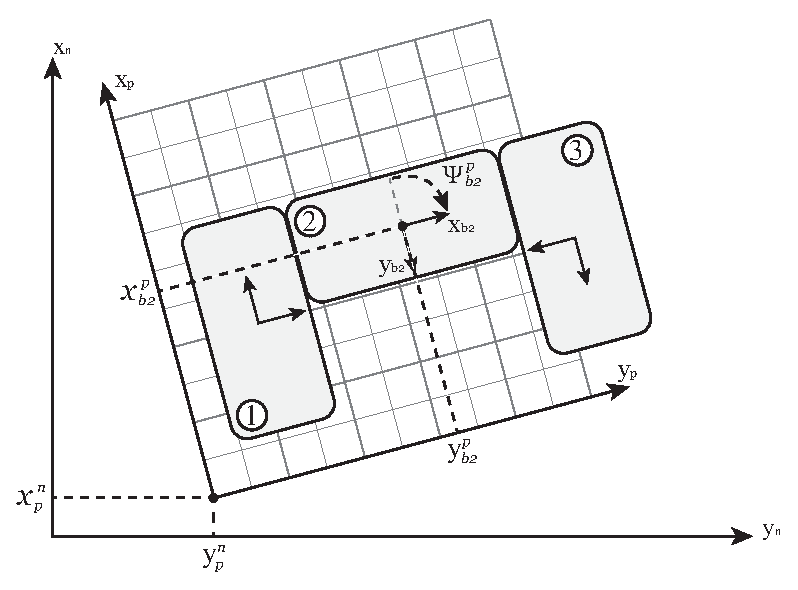
\includegraphics[width=0.8\textwidth]{ned_platform_frame}
	\caption{A platform consisting of three modules. Expression of pose of vessel 2 in the platform coordinate system ($ \{p\}$) is illustrated, as well as position of the platform frame origin in global ($ \{n\}$) frame. This example shows the origin of the platform coordinate system outside of the physical body of the platform, but this placement can be chosen elsewhere at the convenience of the designer.}
	\label{fig:bartned_platform_frame}
\end{figure}

Each module $m_i$ has $r_i = 0,1,2,...$ actuators that are able to impose forces on that module to move it, such as propellers. The amount of actuators that modules have may not be equal for all vessels. This may be unequal by design (as in a heterogenous fleet) , or as a response to a noticed malfunctioning thruster. The total amount of actuators is the summation of the actuators of all vessels.

\begin{equation} 
r =\sum_{i=1}^{n} r_i
\end{equation}

Actuators are bound to various constraints such as direction and maximum force output. Acuators that make forces between vessels to connect them could be described as actuators as well, which can be benificial if connections are not considered rigid. Actuators have dynamics of their own, meaning that they often do not respond instantaneous. However, modelling the dynamics of actuators can  overcomplicate a total system model. If a model is to be kept simple, one can assume that execution of actuator reference is done sufficiently accurate and timely. It is a good idea to reflect if this assumption is reasonable by evaluating the performance of used actuators to accurately follow control inputs, and judge whether inacurracy or delay will significantly affect overall system behavior. 

\subsection{Motion control systems}
Waterborn vehicle dynamics can be described according to \citet{fossen2011handbook}, where the author shows that translational motion of a vessel about CO satisfies

\begin{equation}
m [ \dot{\textbf{v}}_{b/n}^{b} + \dot{\omega}_{b/n}^{b}  \times \textbf{r}_g^b     + \omega_{b/n}^{b}  \times  \textbf{v}_{b/n}^{b} +  \omega_{b/n}^{b}  \times ( \omega_{b/n}^{b}  \times \textbf{r}_g^b   ) ] = \textbf{f}_b^b
\label{eq:fossen2011TranslationalMotionAboutCO-eqnumber-3-33}
\end{equation}

and that rotational motion of a vessel about CO satisfies

\begin{equation} 
\textbf{I}_b  \dot{\omega}_{b/n}^{b} + \omega_{b/n}^{b}  \times \textbf{I}_b \omega_{b/n}^{b}  + m \textbf{r}_g^b \times  ( \dot{\textbf{v}}_{b/n}^{b} +   	\omega_{b/n}^{b} 	 \times	\textbf{v}_{b/n}^{b}	) = \textbf{m}_b^b 
\label{eq:fossen2011RotationalMotionAboutCO-eqnumber-3-40} 
\end{equation}

where components in equation \ref{eq:fossen2011TranslationalMotionAboutCO-eqnumber-3-33} and \ref{eq:fossen2011RotationalMotionAboutCO-eqnumber-3-40} are defined as

\begin{table}[H]
	\centering
	\begin{tabular}{llll}
		$\boldmath{f}^{b}_{b} $ 	   	& = & $[X,Y,Z]^\top$ 		&	- Force with line of action through point $o_b$ expressed in coordinate system $\{b\}$ \\[5pt]
		$\boldmath{m}^{b}_{b} $   		& = & $[K,M,N]^\top$ 		&	- Moment about point $o_b$ expressed in coordinate system $\{b\}$ \\[5pt]
		$ \textbf{v}^{b}_{b/n}$   		& = & $[u,v,w]^\top$ 		&	- Linear velocity of point $o_b$ with respect to $o_n$ expressed in coordinate system $\{b\}$ \\[5pt]
		$ \omega^{b}_{b/n}$   			& = & $[p,q,r]^\top$ 		&	- Angular velocity of $\{b\}$ with respect to $\{n\}$ expressed in coordinate system $\{b\}$  \\[5pt]
		$\textbf{r}^{b}_{g} $ 			& = & $[x_g,y_g,z_g]^\top$ 	&	- Position of centre of gravity expressed in coordinate system $\{b\}$ 
	\end{tabular}
\end{table}

\citet{fossen1994guidance} expresses equation \ref{eq:fossen2011TranslationalMotionAboutCO-eqnumber-3-33} and \ref{eq:fossen2011RotationalMotionAboutCO-eqnumber-3-40} vectorial form
\begin{equation}
\textbf{M}_{RB} \dot{\nu} + \textbf{C}_{RB}(\nu)\nu  = \tau_{RB}
\label{eq:fossen1994RigidBodyKinetics1}
\end{equation}

where $ \textbf{M}_{RB} $ is the rigid body inertia matrix, $\textbf{C}_{RB}$ is a matrix of rigid-body Coriolis and centripetal forces due to the rotation of $\{b\}$ about the inertial frame $\{n\}$, $\nu$ is a vector with generalized velocities expressed in $\{b\}$ and $\tau_{RB}$ is a vector with generalized forces expressed in $\{b\}$. 

Dampening forces can be modelled linear with constant D matrix as 
\begin{equation}
\textbf{M}_{RB} \dot{\nu} + \textbf{C}_{RB}(\nu)\nu  + \textbf{D}\nu = \tau
\label{eq:fossen1994RigidBodyKineticsinclDampeningLinear}
\end{equation}


Or nonlinear as: 
\begin{equation}
\textbf{M}_{RB} \dot{\nu} + \textbf{C}_{RB}(\nu)\nu  + \textbf{D}(\nu)\nu = \tau
\label{eq:fossen1994RigidBodyKineticsinclDampeningNonLinear}
\end{equation}
Which can both be estimated by model identification experiments. Whether linear or nonlinear dampening models are suitable depends on the accuracy of tests and reasonabe operating range. It is common to model some hydrodynamic forces as constant additive accelleration coefficients. \citet{humphreys1978prediction} states that the forces and moments represented by the acceleration hydrodynamic coefficients can, to a very great extent, be modeled as potential flow phenomena, yielding 

\begin{equation}
\textbf{M} \dot{\nu} + \textbf{C}(\nu)\nu  + \textbf{D}(\nu)\nu = \tau{}
\label{eq:fossen1994RigidBodyKineticsinclAddedMass}
\end{equation}

where
\begin{equation}
\textbf{M} = \textbf{M}_{RB} + \textbf{M}_{A}
\end{equation}
Where $ \textbf{M}_{RB} $ represents inertia of the rigid module and $\textbf{M}_{A}$ represents hydrodynamic added mass. Similarly
\begin{equation}
\textbf{C}(\nu)\nu = \textbf{C}_{RB}(\nu)\nu + \textbf{C}_{A}(\nu)\nu
\end{equation}
Where $ \textbf{C}_{RB}(\nu)\nu $ and $\textbf{C}_{A}(\nu)\nu$ represent coriolis and centripetal forces of the rigid body and hydrodynamic added mass. 

Control forces of all actuators (of all modules) can be described in a vector format as:
\begin{equation}
\textbf{f} = [F_{1},F_{2},F_{3}, ... F_{r}]^\top
\end{equation}
Where $F_i$ is the control force generated by actuator $r_i$. 
If the relation between control input and resulting force can be assumed linear, the control forces can be expressed as:

\begin{equation}
\textbf{f} = \textbf{K} * \textbf{u}
\end{equation}

Where $\textbf{u}$ is a vector of control inputs and $\textbf{K}$ is a diagonal force coefficient matrix (see \citet{fossen2011handbook})

Control forces applied across the body can be expressed in total control forces:
\begin{equation}
\tau = \textbf{T}(\alpha)\textbf{f}
\end{equation}
Where $ \textbf{T}(\alpha) \in \mathbb{R}^{n\times r}$ is the thrust configuration matrix, dependent on angles $ \alpha = [\alpha_1,... \alpha_p]^\top \in \mathbb{R}^{p}$ of p rotatable thrusters. \citet{fossen2011handbook} shows how the use of angles of rotatable thrusters can be avoided in the above expression by decoupling the force of a rotatable thruster in two separate forces (generaly decoupled in x and y for surface vessels). Decoupling x and y components of a rotating thruster can simplify math challenges, but does require to take into account physical constraints of absolute maximum thrust of the actuator. 



The team of connected modules has a single, dynamic, multi-robot task, namely the control of actuators to satisfy a time varying platform state. What a satisfactory state actually is depends on the designer, but this is usually defined as a reference state, such as desired positions, and/or velocities.  Utilizing the concept of a reference state in a multi-robot collaborative system means that the controlling entity of a module or platform needs means to aquire the control objective. Various design options are possible to have a set of robots collaborating towards  achieving a single goal. The control objective can be created by various entities.
\begin{itemize}
	\item The robot can generate its own control objective, sensing the environment and following a decision protocol. 
	\item The control objective can be generated by another entity, such as another robot or an operator. This would require means of communication. 
\end{itemize}

\citet{parasuraman2000model} describes an approach on dividing a control problem in four stages with similarities to human decision making. This approach is general and intended to be applicable to a wide spectrum of robot systems, as shown in figure \ref{fig:parasuraman2000model-foursteps}, yet can be applied to a multi-robot system as well. The amount of agents in the multi robot system that collaboratively perform functionality of one of the stages can vary. Some tasks can be done by a single agent, while other tasks can be achieved with multiple. For example; sensing fleet state can be done by a single centralized agent, sending sensor data to on board decision makers, or each vessel can have its own means of sensing its surroundings. 
%\colorbox{yellow}{\parbox{12cm}{This is a very }}\\
%"The first stage refers to the acquisition and registration of multiple sources of information. This stage includes the positioning and orienting of sensory receptors, sensory processing, initial pre-processing of data prior to full perception, and selective attention. The second stage involves conscious perception, and manipulation of processed and retrieved information in working memory [13]. This stage also includes cognitive operations such as rehearsal, integration and inference, but these operations occur prior to the point of decision. The third stage is where decisions are reached based on such cognitive processing. The fourth and final stage involves the implementation of a response or action consistent with the decision choice." \cite{parasuraman2000model}

A collaborative multi vessel control system can thus have its tasks distributed across agents in many ways. To control $n$ vessels where each vessel is equipped with $r_i$ actuators, the following system components can be identified for a certain design divided as shown in \citet{parasuraman2000model}
\begin{itemize}
	\item i agents that aquire information about the state, or called sensing.
	\item j agents that interpret sensed information, converting it into concepts, such as a state estimate. 
	\item k agents that formulate sets of control options
	\item l agents that decide a control option from the set
\end{itemize}

\begin{figure}[H]
	\centering
	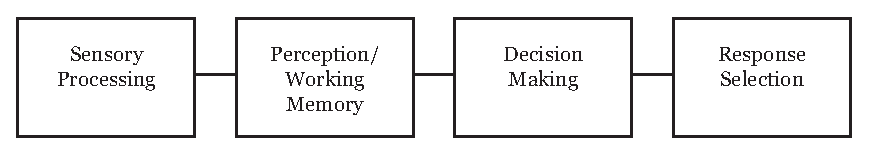
\includegraphics[width=0.8\textwidth]{parasuraman2000model-foursteps}
	\caption{Four-stage model of human information processing. \cite{parasuraman2000model}}
	\label{fig:parasuraman2000model-foursteps}
\end{figure}

Classic marine control theory pertains only a single ship. A common division of the overall control system into subsystems is according to the Guidance, Navigation and Control (GNC) scheme \cite{fossen2011handbook}. The navigation system uses sensors and an observer to generate a state estimate. The guidance system performs task planning and continuously generates a control objective or reference. This is used by the (motion) control system to coordinate responses of available actuators, such that the vessel response follows the reference. 

\subsection{Multi-robot Cooperation}
Various challenges in cooperative multi robot systems are systematically described in existing literature. A section of relevant terms and concepts will be discussed to adress the problem of this section. 

For a multi-robot system, the division of tasks to a set of robots is referred to as "task allocation" \citet{lerman2006analysis}. This is extended to "dynamic task allocation" if the assignment of tasks to robots needs to be adjusted continuously due to changes in task environment and system response. 
\citet{lerman2006analysis} describes a "distributed multi-robot system" as a MRS that does not have a central coordinator. Distribution and centralization of control structure both have their benefits and disadvantages. Decisions in distributed control systems need to be made with incomplete information, while a centralized decision making agent has the potential to use all available data. Centralized control structures have, however, a single point of failure and can encounter scaling issues. 

As multiple robots collaboratively seek to perform the common task of platform motion control, there are varying approaches to allocating control efforts with similar results, as a vessel platforms actuators are likely far more numerous than the (debatably consistent) degrees of freedom. \citet{fossen2011handbook} shows how a vessel motion control block is commonly divided into a dedicated subsystem that generates 'control efforts', and a block that allocates the desired control effort, by dividing it over the available actuators, schematically shown in figure \ref{fig:fossenControlAllocationPNG}. This approach is also used for the configuration adaptive vessel platform controller in \citet{park2019coordinated}, while therein control allocation is referred to as "coordination" and generation of control efforts is referred to as "robust control". 

 \begin{figure}[h!]
 	\centering
 	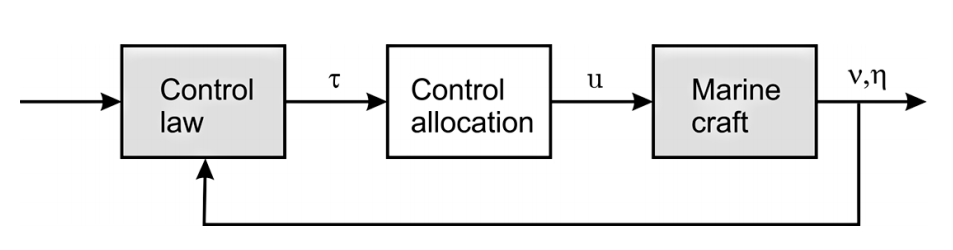
\includegraphics[width=0.6\textwidth]{fossen2011handbookControlAllocation}
 	\caption{Block diagram showing the control-allocation-block in a vessel motion control system. \cite{fossen2011handbook}.}
 	\label{fig:fossenControlAllocationPNG}
 \end{figure}
 
To use this methodology for control of vessel platform motion, the state estimation would need to pertain platform state, and not that of an individual vessel. This is generally positions $\eta_p$ and possibly velocities $\nu_p$, which are to be controlled to a desired state. Which parts of the state are to be controlled depends on the approach and complexity of the control system. Dynamic positioning, for instance, controls pose ($\eta = [x,y,\Psi]$) but not directly velocities ($\nu = [u,v,r]$).

\citet{park2019coordinated} utilizes a centralized control approach to generate control efforts that need to be applied on the platform, while their approach assumes rigid connections. Control effort generation was achieved by means of a PI controller. Control decisions are made centralized on one vessel that is elected as coordinator, which divides the control effort over platform modules. A schematic of the control loop of \citet{park2019coordinated} is  shown in figure \ref{fig:park2019coordinatedSontrolScheme}, showing various elements that could be sensibly interpreted with both the four stage model of \citet{parasuraman2000model} and the GNC scheme as described by \citet{fossen2011handbook}.

\begin{figure}[H]
	\centering
	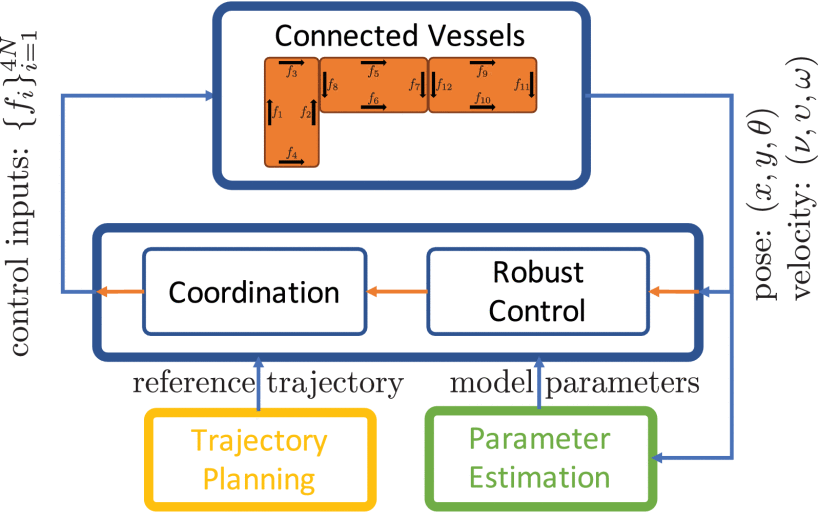
\includegraphics[width=0.6\textwidth]{park2019coordinatedSontrolScheme}
	\caption{Multi-vessel navigation system that consists of parameter estimation, trajectory planning, and coordinated robust control. \cite{park2019coordinated}. Note that the reference trajectory signal is not fed into the coordination block, although it might be interpreted as such on a first glance.}
	\label{fig:park2019coordinatedSontrolScheme}
\end{figure}
\section{Effects of combining systems}
\label{analysisCombined}
The previous sections discussed system analysis of modular surface vessel platforming systems that perform automated reconfiguration (section \ref{analysisReconfiguration}), and configuration adaptive platform control approaches (section \ref{analysisConfigAdaptation}).
This section combines the analysis presented on these two systems by assessing how the functionality of these two systems can be combined. Various design considerations have been identified of which some will be discussed again in this section in a more pragmatic way. Fundamental requirements to achieve the system demands will be presented, yet more emphasis will be given on predicting what choices will be more relevant for commercial logistic applications instead of general robotics. 


\subsection{Requirements}
In order to realize both behaviors, various subfunctions have been identified in section \ref{analysisConfigAdaptation} and \ref{analysisReconfiguration}, which are summarized. Table \ref{tab:assemblyCharacteristicsSummed} presents characteristics of a system that performs Automatic vessel platform reconfiguration, together with the approach and design choices of projects that published about such systems. A similar table on characteristics of vessel platform systems that perform configuration adaptive control strategies are shown in table \ref{tab:adaptiveCharacteristicsSummed}:

\begin{table}[H]
	\centering
	\begin{adjustbox}{width=1\textwidth}
		\begin{tabular}{|l|l|l|l|}
			\hline		
			\begin{tabular}[c]{@{}l@{}}Fundamental Characteristic \\ or requirement \end{tabular} & Roboat project \cite{kelly2019algorithms} \cite{mateos2019autonomous} & \begin{tabular}[c]{@{}l@{}} ISO container module assembly \\ project \cite{o2014self} \cite{paulos2015automated}\end{tabular} & Notes \\ \specialrule{1.5pt}{1pt}{1pt}
			
			A set of modules & Homogeneous fleet  &  Homogeneous fleet  & 	\begin{tabular}[c]{@{}l@{}} Approaches and goals of implementing heterogenous and \\ homogeneous systems differ significantly. \end{tabular} \\ \hline
			
			A strategy to reconfigure. & Deterministic& Deterministic & \begin{tabular}[c]{@{}l@{}}  Various approaches are possible which can be categorized as stochastic \\ or deterministic \end{tabular}\\ \hline
			
			Means of repositioning modules  & \begin{tabular}[c]{@{}l@{}}Cross shaped non roatable\\ thruster setup. Individual \\ vessels are fully actuated \end{tabular} & \begin{tabular}[c]{@{}l@{}}Plus shaped non roatable\\ thruster setup. Individual \\ vessels are fully actuated \end{tabular} & \begin{tabular}[c]{@{}l@{}} Modules can be designed to perform independent or with help from \\ other agents. Individual modules can be under- or fully actuaded, while \\ the observed trend is towards the latter. \end{tabular} \\ \hline
			
			Means of maintaining configuration  & 
			\begin{tabular}[c]{@{}l@{}}Physical ball-cone joint  \\ connection \cite{mateos2019autonomous} or by means \\ of magnets \end{tabular}  &
			\begin{tabular}[c]{@{}l@{}}Physical rope-hook joint \\ connection. Variable \\ stiffness \end{tabular}  & 
			Various solutions are possible, depending on scale, goal and environment. \\ \hline
			
		\end{tabular}
	\end{adjustbox}
	\caption{Fundamental characteristics on automated modular vessel platform reconfiguration systems}
	\label{tab:assemblyCharacteristicsSummed}
\end{table}

\begin{table}[H]
	\centering
	\begin{adjustbox}{width=1\textwidth}
		\begin{tabular}{|l|l|l|}
			\hline		
			\begin{tabular}[c]{@{}l@{}}Fundamental Characteristic \\ or requirement \end{tabular}  & \citet{park2019coordinated}  &  Notes \\ \specialrule{1.5pt}{1pt}{1pt}
			
			Connected robots share a single objective & The platforms position is given as a reference. & \begin{tabular}[c]{@{}l@{}} Other approaches may also attempt to more directly \\ control speed besides position, or integrate higher \\ level planning (e.g. guidance) tasks.\end{tabular} \\ \hline
				
			Robot actions are coordinated  & \begin{tabular}[c]{@{}l@{}} A platform has a centralized controller,\\ deciding and coordinating all connected modules. \end{tabular} & \begin{tabular}[c]{@{}l@{}} Coordinated behavior is aimed to improve\\ performance with respect to the sum of individuals, \\ yet comes at the cost of increased complexity. \end{tabular}\\ \hline
		
			\begin{tabular}[c]{@{}l@{}} The decision making protocol functions\\ on a wide variety of configurations \end{tabular}  & \begin{tabular}[c]{@{}l@{}} Control approach uses an approximate model based \\ on the number of connected modules (however, not \\ the  configuration shape). The control system yields \\ a single control effort for the entire platform that is \\ subsequently distributed among modules. \end{tabular} & \begin{tabular}[c]{@{}l@{}} Criteria of motion control performance will \\ vary between usecases, as well as the amount of\\ considered configurations.   \end{tabular} \\ \hline
			
			
			
		\end{tabular}
	\end{adjustbox}
	\caption{Fundamental characteristics on collaborative and coordinated vessel-platform motion control systems}
	\label{tab:adaptiveCharacteristicsSummed}
\end{table}


An additional characteristic is identified as these two behaviors are integrated in one framework. As a platform configuration changes through time, the motion control system needs to be able to support real time varying configuration parameter, such as estimated dynamics, size, shape, or centre of mass, or in some cases even the network topology. 

\subsection{Common Considerations}
Various considerations for multi robot systems have been observed as key to characterizing a design and are discussed here.

Choosing centralized or decentralized control structures affect many design options for both platform asembly and control. Decentralization generally facilitates great scalability, such that they can be deployed at small scale and in great numbers. A centralized entity can however make decisions based on a more complete state of the overall system, and make more effective decisions. Centralized systems have a single point of failure, which can be undesirable. Centralized systems are also reliant on a communication network with a certain reliability, latency and bandwith.

Homogeneous robot systems consist of robots which are designed to be similar, while heterogeneous systems have modules equipped with different shape, size or abilities. Heterogenous robots can use a wider variety of features without adding too many features per module, although a system topology can get more complex. Homogeneous robots can be interchanged by any other if desired, and are possibly easier to produce in large numbers. All sources that published results on systems that performed automated reconfiguration and configuration adaptive control have been applied using a homogenous fleet.

Vessels that operate individually can be underactuated or fully actuated. Control of underactuated systems is generally more complex, though not impossible. \citet{ashrafiuon2010review} reviews different approaches of controlling automated  underactuated surface vessels. This work focusses on control approaches which are categorized in "setpoint", "trajectory tracking" and "path following" approaches. Light is shed on advantages and disadvantages of various mentioned approaches. It is convenient to have fully actuated modules for vessel platforming purposes, which is shown to be feasible by projects that use fully actuated vessels for both automated reconfiguration and configuration adaptive control. 

Designing towards utilizing extensive amounts of communication in a multi robot system drastically changes availability of further design options. A vessel system connected into a network that continuously shares information can become reliant on the presence and performance of the network. Facilitating connectivity comes to cost at various facets. Modules need this extra feature built in, which makes a module more complex, expensive, power consuming, while adding another component that can break. Nihilistic approaches that only add essential features to a module will increase scalability, due to low cost, replacability and reliability. 


To facilitate collaborative platform control, some communication between operator and module is always necessary, as the task of the platform needs to be communicated from human to the vessel system. Many multi robot systems that are nowadays developed often have a high reliance on communication network availability, as task distribution has many benefits and opens up new doors in terms of design choices and possible emergent behaviors. 

\vspace{5mm}

This chapter explored the meaning two behaviors of automated vessel platform control systems reffered to as 'automated reconfiguration' and 'collaborative and coordinated platform motion control'. Various approaches to describing and designing such systems were discussed to deepen understanding of the behaviors and broaden the view on potential design solutions. Fundamental characteristics of both evaluated systems have been identified to aid development of a framework integrating the two in the next chapter. 






